%% %% %% %%
%%
%% Parte A de la práctica
%%
%% %% %% %%

\documentclass[../procedimientos.tex]{subfiles}
\graphicspath{{\subfix{../../images/}}}

\begin{document}
\clearpage
\subsection{Parte A}
\subsubsection{Instrucciones}
\begin{em}
  Programar las funciones mostradas, en un formato SOP y POS mínimo (reducido) 
  en forma flujo de datos, para su posterior simulación dentro de la 
  plataforma \textit{Quartus II}.
  \begin{itemize}
    \item \textbf{Mediante POS}
      \begin{equation*}
        f(xyzt) = (x + \n{x}y + \overline{yt})(x + \overline{xy}\cdot z)
      \end{equation*}
    \item \textbf{Mediante SOP}
      \begin{equation*}
        f(uvtw) = vt(u+t\n{w})(u+\n{w})+wu(v+t)
      \end{equation*}
  \end{itemize}
\end{em}

\subsubsection{Análisis}\label{subs:analisis_a}
Primero, se desarrollará la función $f(xyzt)$ a través de álgebra booleana 
para encontrar una forma POS reducida:
\begin{align*}
  f(xyzt) &= (x + \n{x}y + \overline{yt})(x + \overline{xy}\cdot z)\\
  &= (\cancel{(x+\n{x})}(x+y) + \overline{yt})(x + (\n{x}+\n{y})z)\\
  &= \cancel{(x+y + \n{y} + \n{t})}(x + (\n{x}+\n{y})z)\\
  &= \cancel{(x+\n{x}+\n{y})}(x+z)\\
  &= (x+z)
\end{align*}
\begin{equation*}
  \boxed{
    \therefore f(xyzt) = (x+z)
  }
\end{equation*}

Posteriormente, se desarrollará la función $f(wvtw)$ a través de álgebra 
booleana para encontrar una forma SOP reducida:
\begin{align*}
  f(uvtw) &= vt(u+t\n{w})(u+\n{w})+wu(v+t)\\
  &= vt(u+t)(u+\n{w})\cancel{(u+\n{w})}+wu(v+t)\\
  &= vt(u+t)(u+\n{w})+wu(v+t)\\
  &= vt(u+t\n{w})+wuv+wut\\
  &= uvt+vt\n{w}+uvw+utw
\end{align*}
\begin{equation*}
  \boxed{
    \therefore f(uvtw) = uvt+vt\n{w}+uvw+utw
  }
\end{equation*}

\subsubsection{Implementación en Quartus}\label{subs:a_imp}
Con las formas reducidas anteriormente, se implementó el sistema dentro de la 
plataforma \textit{Quartus II}. Para esto, después de crear el proyecto, se 
creó un nuevo archivo de tipo \textbf{VHDL}, el cual tiene el contenido 
mostrado a continuación:
\begin{lstlisting}[language=VHDL, caption=Archivo VHDL (Parte A)]
-- Implementacion: Parte A

library ieee;
use ieee.std_logic_1164.all;

entity p04a is
	port (
		a, b, c, d		: in		std_logic;
    f1, f2			  : out		std_logic
	);
end;

architecture simple of rlg_p04a is
begin
	f1 <= a or c;
  f2 <= (a and b and c) or (b and c and not d)
        or (a and b and d) or (a and c);
end;
\end{lstlisting}

En este caso, para poder ejecutar ambas funciones se renombraron sus entradas 
de la siguiente forma:
\begin{itemize}
  \item Para $f(xyzt)$: $f_1(abcd)$
    \begin{itemize}
        \item $x$: $a$
        \item $y$: $b$
        \item $z$: $c$
        \item $t$: $d$
    \end{itemize}
  \item Para $f(uvtw)$: $f_2(abcd)$
    \begin{itemize}
        \item $u$: $a$
        \item $v$: $b$
        \item $t$: $c$
        \item $w$: $d$
    \end{itemize}
\end{itemize}

Que es justo lo que se puede apreciar en el código. Para continuar, se simuló 
el circuito dentro de la misma plataforma, a través de una simulación 
funcional. Se obtuvieron las siguientes salidas:
\begin{figure}[H]
  \centering
  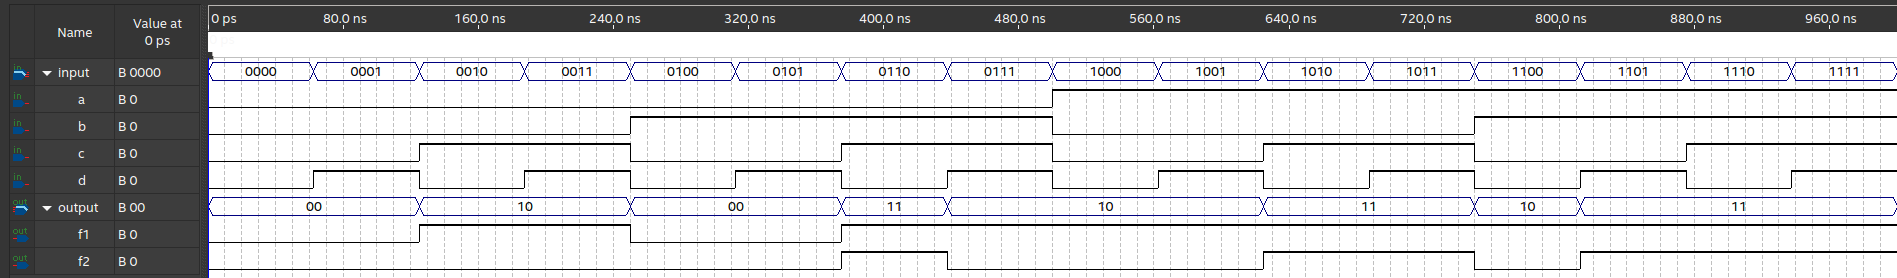
\includegraphics[width=\textwidth]{sim_a}
  \caption{Simulación Funcional (Parte A)}
\end{figure}

El resultado obtenido coincide con el comportamiento de ambas funciones 
$f(xyzt)$ y $f(uvtw)$.
\end{document}

